\documentclass[a4paper,12pt]{article}
\usepackage[a4paper, top=2cm,bottom=2cm,right=2cm,left=2cm]{geometry}

\usepackage{bm,xcolor,mathdots,latexsym,amsfonts,amsthm,amsmath,
					mathrsfs,graphicx,cancel,tikz-cd,hyperref,booktabs,caption,amssymb,amssymb,wasysym}
\hypersetup{colorlinks=true,linkcolor=blue}
\usepackage[italian]{babel}
\usepackage[T1]{fontenc}
\usepackage[utf8]{inputenc}
\newcommand{\s}[1]{\left\{ #1 \right\}}
\newcommand{\sbarra}{\backslash} %% \ 
\newcommand{\ds}{\displaystyle} 
\newcommand{\alla}{^}  
\newcommand{\implica}{\Rightarrow}
\newcommand{\iimplica}{\Leftarrow}
\newcommand{\ses}{\Leftrightarrow} %se e solo se
\newcommand{\tc}{\quad \text{ t. c .} \quad } % tale che 
\newcommand{\spazio}{\vspace{0.5 cm}}
\newcommand{\bbianco}{\textcolor{white}{,}}
\newcommand{\bianco}{\textcolor{white}{,} \\}% per andare a capo dopo 																					definizioni teoremi ...


% campi 
\newcommand{\N}{\mathbb{N}} 
\newcommand{\R}{\mathbb{R}}
\newcommand{\Q}{\mathbb{Q}}
\newcommand{\Z}{\mathbb{Z}}
\newcommand{\K}{\mathbb{K}} 
\newcommand{\C}{\mathbb{C}}
\newcommand{\F}{\mathbb{F}}
\newcommand{\p}{\mathbb{P}}

%GEOMETRIA
\newcommand{\B}{\mathfrak{B}} %Base B
\newcommand{\D}{\mathfrak{D}}%Base D
\newcommand{\RR}{\mathfrak{R}}%Base R 
\newcommand{\Can}{\mathfrak{C}}%Base canonica
\newcommand{\Rif}{\mathfrak{R}}%Riferimento affine
\newcommand{\AB}{M_\D ^\B }% matrice applicazione rispetto alla base B e D 
\newcommand{\vett}{\overrightarrow}
\newcommand{\sd}{\sim_{SD}}%relazione sx dx
\newcommand{\nvett}{v_1, \, \dots , \, v_n} % v1 ... vn
\newcommand{\ncomb}{a_1 v_1 + \dots + a_n v_n} %a1 v1 + ... +an vn
\newcommand{\nrif}{P_1, \cdots , P_n} 
\newcommand{\bidu}{\left( V^\star \right)^\star}

\newcommand{\udis}{\amalg}
\newcommand{\ric}{\mathfrak{U}}
\newcommand{\inclu}{\hookrightarrow }
%ALGEBRA

\newcommand{\semidir}{\rtimes}%semidiretto
\newcommand{\W}{\Omega}
\newcommand{\norma}{\vert \vert }
\newcommand{\bignormal}{\left\vert \left\vert}
\newcommand{\bignormar}{\right\vert \right\vert}
\newcommand{\normale}{\triangleleft}
\newcommand{\nnorma}{\vert \vert \, \cdot \, \vert \vert}
\newcommand{\dt}{\, \mathrm{d}t}
\newcommand{\dz}{\, \mathrm{d}z}
\newcommand{\dx}{\, \mathrm{d}x}
\newcommand{\dy}{\, \mathrm{d}y}
\newcommand{\amma}{\gamma}
\newcommand{\inv}[1]{#1^{-1}}
\newcommand{\az}{\centerdot}
\newcommand{\ammasol}[1]{\tilde{\gamma}_{\tilde{#1}}}
\newcommand{\pror}[1]{\mathbb{P}^#1 (\R)}
\newcommand{\proc}[1]{\mathbb{P}^#1(\C)}
\newcommand{\sol}[2]{\widetilde{#1}_{\widetilde{#2}}}
\newcommand{\bsol}[3]{\left(\widetilde{#1}\right)_{\widetilde{#2}_{#3}}}
\newcommand{\norm}[1]{\left\vert\left\vert #1 \right\vert \right\vert}
\newcommand{\abs}[1]{\left\vert #1 \right\vert }
\newcommand{\ris}[2]{#1_{\vert #2}}
\newcommand{\vp}{\varphi}
\newcommand{\vt}{\vartheta}
\newcommand{\wt}[1]{\widetilde{#1}}
\newcommand{\pr}[2]{\frac{\partial \, #1}{\partial\, #2}}%derivata parziale
%per creare teoremi, dimostrazioni ... 
\theoremstyle{plain}
\newtheorem{thm}{Teorema}[section] 
\newtheorem{ese}[thm]{Esempio} 
\newtheorem{ex}[thm]{Esercizio} 
\newtheorem{fatti}[thm]{Fatti}
\newtheorem{fatto}[thm]{Fatto}

\newtheorem{cor}[thm]{Corollario} 
\newtheorem{lem}[thm]{Lemma} 
\newtheorem{al}[thm]{Algoritmo}
\newtheorem{prop}[thm]{Proposizione} 
\theoremstyle{definition} 
\newtheorem{defn}{Definizione}[section] 
\newcommand{\intt}[2]{int_{#1}^{#2}}
\theoremstyle{remark} 
\newtheorem{oss}{Osservazione} 
\newcommand{\di }{\, \mathrm{d}}
\newcommand{\tonde}[1]{\left( #1 \right)}
\newcommand{\quadre}[1]{\left[ #1 \right]}
\newcommand{\w}{\omega}

% diagrammi commutativi tikzcd
% per leggere la documentazione texdoc

\begin{document}
\textbf{Lezione del 11 Marzo e prima parte della lezione del 12  Marzo}
\begin{thm}[di classificazione]\bianco 
Le superfici compatte e orientabili (qualsiasi cosa voglia dire) sono tutte e sole le seguenti $\Sigma_i$ \\
dove $\Sigma_i$ \`e la superficie con $i$-buchi
\end{thm}
\begin{oss}$\Sigma_0=S^2$ (la sfera) mentre $\Sigma_1=S^1 \times S^1$ (il toro)
\end{oss}
Calcoliamo il $\pi_1$ del toro usando il teorema di Van Kamper
Sia $Q$ il quadrato e sia $p$ il centro del quadrato.\\
Il toro si ottiene identificando i lati opposti del quadrato, sia $\pi:\, Q \to \Sigma_1$ la proiezione al quoziente.\\
Siano $A=\pi(Q\sbarra \{p\}$ e $B =\pi(Q \sbarra \partial Q)$ da cui $A\cap B = \pi( Q \sbarra (\{ p\} \cup \partial Q)$\\
Osserviamo che $A,B$ e $A \cap B$ sono aperti (essendo immagine di aperti saturi) e connessi per archi.\\
Ora $Q\sbarra \{p\}$ si retrae a $\partial Q$ che a sua volta si proietta su $S^1 \wedge S^1$, la retrazione passa al quoziente, $A$ si ritrae su $S^1 \wedge S^1$, abbbiamo $\pi_1(A)= \Z \star \Z$ con generatori $a,b$\\
Osserviamo che $B$ \`e omeomorfo a $Q\sbarra \partial Q $ ($\pi_{Q\sbarra \partial Q}$ \`e l'omomorfismo cercato), poich\`e tale insieme \`e convesso si ha $\pi_1(B)=1$\\
Ora $A\cap B$ si ritrae su $S^1$ percui $\pi(A\cap B)=\Z$\\
Abbiamo dunque il seguente diagramma 
 $$ \begin{tikzcd}
 & \pi_1(A) \arrow[dr] \\ \pi_1(A\cap B) \arrow{ur}{\phi}  \arrow{rd}{\psi}& &\pi_1(\Sigma_1)\\& \pi_1(B) \arrow[ur]
\end{tikzcd}  \, \, \,  \begin{tikzcd}
 & \Z\star \Z \arrow[dr] \\ \Z \arrow{ur}{\phi}  \arrow{rd}{\psi}& &\pi_1(\Sigma_1)\\& \{ 1 \} \arrow[ur]
\end{tikzcd}$$ 
Ora se $\alpha$ \`e il generatore di $\pi_1(A\cup B)$ disegnato allora $\phi(\alpha)=ab\inv a \inv b$ mentre $\psi$ \`e banale.\\ Dal teorema di Van Kampen si ha $$\pi_1(\Sigma_1)=\frac{\pi_1(A)\star \pi_1(B)}{\phi(\alpha)=\psi(\alpha)} = \langle a,b \, \vert \, ab \inv a \inv b \rangle = \Z \oplus \Z$$
\begin{figure}[!h]
\centering
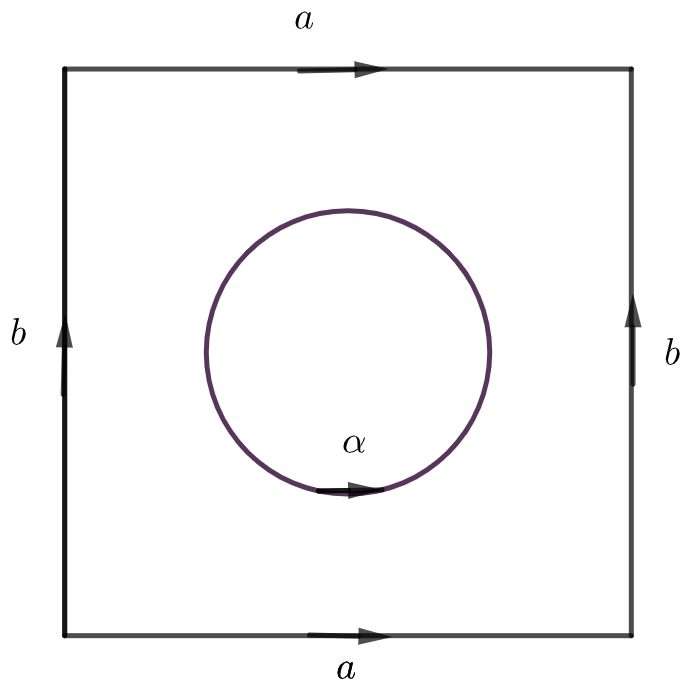
\includegraphics[scale=0.5]{toro}

\end{figure}
\newpage
Possiamo fare una dimostrazione analoga anche per la superficie di genere $2$.\\
Sia $P$ l'ottagono e $p$ il suo centro, sia $\pi:\, P \to \Sigma_2$ identificando i lati con le stesse lettere (vedi disegno)\\
Sia $A=\pi(P\sbarra \{p\})$ e $B=\pi(P\sbarra \partial P)$\\
Come nel caso precedente $A,B$ e $A\cap B$ sono aperti e connessi per archi, $A$ si ritrae su $\pi(\partial P)$ che \`e un boquet di $4$ copie di $S^1$, date dalle proiezioni di $a,b,c,d$, dunque $\pi_1(A)=\Z\star \Z\star \Z\star \Z$.\\
Ora $B$ \`e semplicemente connesso, mentre un convesso di $R^2$ meno un punto interno \`e omotopicamente equivalente a $S^1$ da cui $\pi_1(A\cup B)=\Z$\\
Se $\alpha$ \`e un generatore di $\pi_1(A\cup B) $ allora $\phi(\alpha)= ab\inv a\inv b c d \inv c \inv d $.\\
Per il teorema di Van Kamper si ha 
$$ \pi_1(\Sigma_2)=\langle a,b,c,d \, \vert \, ab\inv a\inv b c d \inv c \inv d \rangle$$\\
\\
Con un procedimento analogo partendo da un $4g$-agono si mostra che 
$$\pi_1(\Sigma_g) =\langle a_1, b_1, \dots, a_g, b_g \, \left\vert \prod_{i=1}^g [ a_i,b_i] \right. \rangle$$
Denotiamo con $\Gamma_g = \pi ( \Sigma_g)$
\begin{thm}
$$\frac{\Gamma_g}{[\Gamma_g,\Gamma_g]} \cong \Z^{2g}$$
\proof Definisco una mappa $\psi :\, \Gamma_g \to \Z^{2g}$ ponendo $\psi(a_i)=e_i$ e $\psi(b_i)=e_{2i+1}$\\
La buona definizione deriva dal fatto che ovviamente le relazioni vadano nell'identit\`a di $Z^{2g}$.\\
Poich\`e $\Z^{2g}$ \`e abeliano si ha $[\Gamma_g,\Gamma_g]\subseteq \ker \psi$ da cui $\psi $ induce 
$$ \overline{\psi}:\, \frac{\Gamma_g}{[\Gamma_g, \Gamma_g]} \to \Z^{2g}$$
Per concludere esibiamo un'inversa di $\overline{\psi}$
$$ \phi :\, \Z^{2g} \to  \frac{\Gamma_g}{[\Gamma_g, \Gamma_g]}  \text{ con } \phi(e_i)=\begin{cases}[[a_i]] \text{ se } i\leq g\\
[[b_i]]\text{ se } i>g \end{cases}$$
Dal fatto che $\frac{\Gamma_g}{[\Gamma_g,\Gamma_g]}$ \`e abeliano, \`e facile verificare che $\phi$ si estende ad un omo di gruppi che \`e l'inversa di $\psi$
\end{thm}
\spazio
\begin{oss}$\Z^m \cong \Z^n \, \ses \, m=n$\\
Infatti se $\varphi:\, \Z^n \to \Z^m$ \`e un omomorfismo, viene rappresentata da una matrice $A$ di taglia $m \times n$.\\
se $\psi:\, \Z^m \to\Z^n$ \`e l'inversa allora viene rappresentata da una matrice $B$ di taglia $n \times m$\\
Ora $AB=I_m$ mentre $BA=I_n$, per fatti noti di algebra lineare si ha $n=m$
\end{oss}
\begin{cor}\bbianco
\begin{itemize}
\item $\Gamma_g \cong \Gamma_{g'} \, \, \ses \, \, g=g'$
\item $\Sigma_g$ \`e omotopicamente equivalente a $\Sigma_{g'}$ se e solo se $g=g'$
\item $\Sigma_g \cong \Sigma_{g'} \, \, \ses \, \, g=g'$
\end{itemize}
\end{cor}

\newpage
D'ora in poi tutti gli spazi saranno localmente connessi per archi 
\begin{prop}Sia $p:\, E\to X$ un rivestimento connesso ($E$ connesso dunque connesso per archi ($E$ localmente connesso).\\
Sia $\tilde{x_0}\in F = \inv p(x_0)$ e sia $\psi:\, \pi_1(X,x_0) \to F$ dove $\psi(\alpha)= \tilde{x_0}\az \alpha$.\\
Allora $\psi$ induce una bigezione tra 
$$ \frac{p_\star(\pi_1(E,\tilde{x_0})}{\pi_(1)(X,x_0)} \to F$$
In particolare $Stab(\tilde{x_0}) = p_\star(\pi_1(E, \tilde{x_0}))$ e al variare di $\tilde{x}\in F$ i gruppi $p_\star ( \pi_1(E,\tilde{x}))= Stab(\tilde{x})$ sono tutti e soli i coniugati di $p_\star(\pi_1(E, \tilde{x_0}))$
\proof Poich\`e $E$ \`e connesso, l'azione di monodromia \`e transitiva, da cui segue la surgettivita di $\psi$\\
Sia $\alpha=[\gamma] \in Stab(\tilde{x_0})$ dunque per definizione di monodromia 
$$\sol{\gamma}{x_0}(1)=\tilde{x_0} \, \, \ses \, \, \sol{\gamma}{x_0} \text{ \`e un loop in } E \, \, \ses \, \, [\gamma] \in p_\star (\pi_1(E, \tilde{x_0}))$$
da ci\`o segue che 
$$ \psi(\alpha)=\psi(\beta)\, \, \ses \, \, \tilde{x_0}\az \alpha = \tilde{x_0}\az\beta \, \, \ses \,\, \tilde{x_0}\az (\alpha \inv \beta ) =\tilde{x_0}\, \, \ses \,\, \alpha\inv\beta \in Stab(\tilde{x_0}) \, \, \ses \, \, [\alpha]=[\beta] \text{ in } \frac{\pi_1(X,x_0)}{Stab(\tilde{x_0})}$$
dunque $\psi$ induce la bigezione cercata.\\
Usando il fatto che l'azione \`e transitiva, \`e facile vedere che $Stab(\tilde{x})$ al variare di $\tilde{x}$ sono tutti e soli i coniugati di $Stab(\tilde{x_0})$ (se $\tilde{x}\in F$ allora $\tilde{x}=\tilde{x_0}\az \eta $ E $Stab(\tilde{x})$ \`e il coniugato di $Stab(\tilde{x_0})$ per $\eta$
\endproof
\end{prop}
\begin{thm}[di sollevamento di mappe]\bianco 
Sia $p:\, E \to X$ un rivestimento connesso, $x_0\in X$, $\tilde{x_0}\in \inv p(x_0)$ e sia $f:\, Y \to X$ continua con $Y$ connesso e sia $y_0\in Y$
$$ \exists \tilde{f}:\, Y \to E \text{ sollevamento di } f \text{ con } \tilde{f}(y)=\tilde{x_0}\,\, \ses \, \, f_\star(\pi_1(Y,y_0))\subset \pi_\star(\pi(E,\tilde{x_0}))$$
\proof $\implica$ se $f=p\circ \tilde{f}$ allora $f_\star=p_\star \circ \tilde{f}_\star$ dunque $Im_{f_\star}\subseteq Im_{p\star}$\\
$\iimplica$ Definiamo $\tilde{f}$ come segue, se $y \in Y$, scegliamo un cammino $\gamma$ in $Y$ che collega $y_0$ a $y$ e poniamo $\tilde{f}(y)= \bsol{f\circ \gamma}{x_0}(1) $.\\
Verifichiamo la buona definizione ovvero che la funzione non dipende dal cammino scelto. Se $\beta$ \`e un altro cammino allora $\gamma\sim \gamma \star \overline{\beta}\star \beta$ come cammini dunque 
$$ f \circ \gamma \sim [ f \circ ( \gamma \star \overline{\beta}\star \beta ) ] = f \circ (\gamma \star \overline{\beta}) \star f\circ \beta $$
Osserviamo che $\alpha=\gamma \star \overline{\beta}$ \`e un loop basato inn $y_0$ da cui  $[f\circ  \alpha]\in f_\star (\pi_1(Y,y_0))\subseteq p_\star (\pi_1(E, \tilde{x_0}))$ dunque $f\circ \alpha$ si solleva ad un loop in $E$ a partire da $\tilde{x_0}$.\\
Si ha dunque 
$$\bsol{f\circ \gamma}x 0(1)=\bsol{(f \circ \alpha)\star (f \circ \beta)}{x} 0 (1)= \bsol{f\circ \alpha}x 0  \star \left(\widetilde{f\star \beta } \right)_{\bsol{f\star \alpha} x 0 (1)}(1)$$
Essendo  $\bsol{f\star \alpha} x 0 $ un loop allora $\bsol{f\star \alpha} x 0(1)=\tilde{x}_0$ da cui
$$\bsol{f\circ \gamma}x 0(1)=\bsol{f\star \beta } x 0 (1)$$
questo mostra la ben definizione di $\tilde{f}$\\
Mostriamo adesso la continuit\`a.\\
Dato $y \in Y$. Sia $U$ intorno aperto ben rivestito di $f(y)\in X$ dunque $\inv p (U) =\prod V_i$ con $V_i $ aperto in $E$.\\
Sia $i_0$ tale che $\tilde{f}(y) \in V_{i_0}$ e sia $s:\, U \to V_{i_0}$ l'inversa continua di $p_{\vert V_{i_o}}$ (esiste per definizione di intorno ben rivestito).\\
Sia $W=\inv f(U)$ che \`e aperto di $Y$ (a meno di prendere un suo sottoinsieme, lo assumo connesso per archi).\\
Per mostrare la continuit\`a di $\tilde{f}$ basta osservare che $\tilde{f}_{\vert W} = s \circ f_{\vert W} $\\ 
Sia $\gamma\in \Omega(y_0, y)$ e $z\in W$ tale che $\gamma_z \in \Omega(y,z)$, per definire $\tilde{f}(z)$ uso il cammino $\alpha_z= \gamma \star \gamma_z$ dunque
$$ \tilde{f}(z)= \bsol{f \circ \alpha_z}x 0 (1) = \bsol{(f\circ \gamma) \star (f\circ \gamma_z)}x 0 (1) = \bsol{f\star \gamma}x 0 \star \left(\widetilde{f\circ \gamma_z}\right)_{\tilde{f}(y)}(1)$$
in quanto $\tilde{f}(y)= \bsol{f\circ \gamma} x 0 (1) $ dunque otteniamo 
$$\bsol{f\circ \gamma}x 0 (1) =  \left( \widetilde{f \circ \gamma_z}\right)_{\tilde{f}(y)} = (s \circ(f\circ \gamma_z))(1)=s(f(z))$$
dove la penultima uguaglianza deriva dall'unicit\`a del sollevamento in quanto $s\circ f \circ \gamma_z$ solleva $f\circ \gamma_z$ a partire da $\tilde{f}(y)$
\endproof
\end{thm}
\begin{cor} Sia $p:\, E \to X$ un rivestimento connesso, $x_0\in X$ e $\tilde{x}_0\in \inv p (x_0)$.
Sia $f:\, Y \to X$ con $f(y_0)=x_0$.\\
Se $Y$ \`e semplicemente connesso $\exists ! \, \tilde{f}:\, Y \to E $ con $\tilde{f}(y_0)=\tilde{x}_0$
\proof La condizione del teorema \`e banalmente vera
\end{cor}
\begin{thm}[di Barsuk-Ulam] Non esistono mappe continue  $f:\, S^2 \to S^1 $ con $f(-x)=-f(x)$
\proof Supponiamo, per assurdo che esista una mappa $f$ come nelle ipotesi.\\
Siano $p:\, S^2 \to \mathbb{P}^2(\R)$ e $q:\, S^1 \to \mathbb{P}(\R)$ le proiezioni al quoziente. Abbiamo, dunque, un diagramma commutativo di funzioni continue
$$\begin{tikzcd}
S^2 \arrow[r,"f"] \arrow[d,"p"] & S^1 \arrow[d,"q"] \\
\mathbb{P}^2(\R) \arrow[dashed]{r}{\overline{f}} &\mathbb{P}(\R)
\end{tikzcd}$$
Ora $\pi_1(\pror2) =\Z_2$ e $\pi_1(\pror 1 )=\Z$ segue che $\overline{f}_\star$ \`e la mappa banale (non esistono omomorfismi non banali da $\Z_2 \to \Z$)\\
Per il teorema di sollevamento $\exists h:\, \pror 2 \to S^1 $ con $q \circ h = \overline{f}$ (non sappiamo che $h\circ p = f$)\\
Scelgo $x_0\in S^2$. So che $ q(h(p(x_0))=q(f(x_0))$ in quanto $q(h(p(x_0))=\overline{f}(p(x_0))= q(f(x_0))$.\\
Dunque $h\circ p $ e $f$ sono sollevamenti di $\overline{f}\circ p$.\\
Sia $z_0 \in \pror 1 $ allora $z_0 =\overline{f}(p(z_0))$.\\
Ora $\inv q (z_0)=\{ y_0, -y_0\}$ dunque posso supporre $f(x_0)=y_0$ e $f(-x_0)=-y_0$.\\
Anche $h(p(x_0)), h(p(-x_0))$ appartengono a $\{ y_0, -y_0\}$ ma $p(x_0)=p(-x_0)$ per cui $h(p(x_0))=h(p(-x_0))$ dunque deve succedere che $f$ e $h\circ p $ coincidono su un punto o $x_0$ o $-x_0$.\\
Ora $f$  e $h \circ p $ sono sollevamenti che coincidono in un punto, per un unicit\`a ($S^2$ connesso) $f=h \circ p $. Ci\`o \`e assurdo in quanto $f(x_0)\neq f(-x_0)$ mentre $h(p(x_0))=h(p(-x_0))$
\endproof
\end{thm}
\begin{cor}$f:\, S^2 \to \R^2$ continua. Allora $\exists x \in S^2 $ con $f(x)=f(-x)$
\proof Se $f(x)\neq f(-x)\, \, \forall x \in S^2$, allora la mappa $g:\, S^2 \to S^1$ definita come 
$$ g(x)=\frac{f(x)-f(-x)}{\norm{f(x)-f(-x)}}$$ 
sarebbe ben definita e continua (il denominatore non si annullano).\\
Tale mappa genera un assurdo perch\`e $g(x)=-g(-x)$
\end{cor}
\begin{cor}In un fissato istante, sulla superficie terrestre, esistono 2 punti antipodali con la stessa temperatura e pressione (che si assumono continue)
\end{cor}
\end{document}